% Dokumentenart festlegen
%Schriftgröße 12pt, A4, mit titelseite,doppelseitig,aber halbseiten überspringen,doppelseiten leer(ohne header)
%\documentclass[12pt,a4paper,titlepage,parskip=half,twoside,cleardoublepage=plain]{scrreprt}
\documentclass[12pt,a4paper,titlepage,parskip=half,cleardoublepage=plain]{scrreprt}
\usepackage[left=35mm,right=20mm,head=15mm,bottom=15mm,includefoot]{geometry}
%\usepackage{geometry}

% Dokumenteninformationen
\title{TEMPLATE}

%export author and title to use later
\makeatletter
\let\thetitle\@title
\let\theauthor\@author
\makeatother





\usepackage[utf8]{inputenc}
\usepackage[T1]{fontenc}

%\usepackage[scaled]{uarial}


%use serif font
\renewcommand*\familydefault{\rmdefault}
%use san serif font
%\renewcommand*\familydefault{\sfdefault}

% Farben festlegen
\usepackage{xcolor}
\definecolor{black}{rgb}{0.0,0.0,0.0}

% Packet für bessere Listen vorallem Kompakte
\usepackage{paralist}


% Bilder einfügen
\usepackage{graphicx}

% Bilder fest positionieren
\usepackage{float}

% Fußnotenzähler durchgängig
\usepackage{chngcntr}
%\counterwithout{footnote}{chapter}

\usepackage{perpage} %the perpage package
\MakePerPage{footnote} %the perpage package command



% Deutsche Übersetzungen automatisch eingefügter Worte
\usepackage[ngerman]{babel}

% Acronyme bzw. Abkürzungen
\usepackage[printonlyused]{acronym}

%\usepackage{relsize}
%\usepackage{xcolor}
%\renewcommand{\bflabel}[1]{#1\hfill}
\renewcommand{\bflabel}[1]{\normalfont{\normalsize{#1}}\hfill}
% kursiv long
\renewcommand*{\acffont}[1]{{\color{black}\itshape{#1}}}
\renewcommand*{\acfsfont}[1]{\textnormal{#1}}

% Subfigure
\usepackage{subfigure}

% Advanced tables
\usepackage{tabularx}

%\usepackage[perpage]{footmisc}

%package for odd pages check
\usepackage{changepage}
\strictpagecheck


\definecolor{listing_bg}{rgb}	{0.98,0.98,0.98}

% Listing package (Code,...)
\usepackage{listings}
\lstloadlanguages{Java}
\lstset{
	basicstyle			= \footnotesize,
	frame						= trLB, 							% Rahmen (right, bottom, left, top; uppercase: double frame)
	breaklines			= true, 							% Zeilenumbruch
	numbers					= left, 							% Zeilennummernformatierung: Schriftausrichtung
	numberstyle			= \tiny, 							% Zeilennummernformatierung: Schriftgroesse
	backgroundcolor	= \color{listing_bg}, % Hintergrundfarbe
	tabsize					= 2, 									% col1 = n+1, col2 = 2n+1
	extendedchars		= true 								% Sonderzeichen
}

%booleans und vergleiche
\usepackage{ifthen}


% Eigene Befehle
\newcommand{\template}{\textit{template}}




\newboolean{commentenabled} %Deklaration
\setboolean{commentenabled}{true} %Enable or disable comments

\newcommand{\comment}[1]{\ifthenelse{\boolean{commentenabled}}{{\color{red}\Huge \bf --------------------\\#1\\--------------------\\}}{}}
\newcommand{\emptypage}{\newpage \thispagestyle{empty} \quad}
\newcommand{\subsubref}[1]{\ref{#1} \textit{\nameref{#1}}}

\newcommand{\cancel}[2]{{\color{red}\sout{#1}{\textbf{#2}}}}

\newcommand{\hierweiter}[0]{\comment{Hier Weiter}}


% Abkürzungen
\newcommand{\bzw}{\mbox{bzw.}}


% Meta Information festlegen IMPORT LAST
\usepackage[
    pdftitle={TEMPLATE},
    pdfsubject={\thetitle},
    pdfauthor={\theauthor},
    pdfkeywords={\thetitle, TEMPLATE}
]{hyperref}

%  Grafiken richtig verlinken
\usepackage[all]{hypcap}





% Links richtig färben
\hypersetup{
	linkcolor		= black,	% red 		Color for normal internal links. 
	anchorcolor		= black,	% black 	Color for anchor text. 
	citecolor		= black,	% green 	Color for bibliographical citations in text. 
	filecolor		= black,	% magenta	Color for URLs which open local files. 
	menucolor		= black,	% red 		Color for Acrobat menu items. 
	urlcolor		= black,	% cyan 		Color for linked URLs.
	colorlinks		= true		% Use colored text instead of a frame around it.
	}
	
\usepackage{textcomp}

% Dicke horizontale Linien mit \Xhline{2\arrayrulewidth}
\usepackage{makecell}

\usepackage{fancyhdr}

\fancypagestyle{basicstyle}{%
  \fancyhf{}
  \fancyhead[LE,RO]{\nouppercase\rightmark}
  \fancyfoot[LE,RO]{\thepage}
  \renewcommand{\headrulewidth}{0.4pt}
  \renewcommand{\footrulewidth}{0pt}}
\pagestyle{basicstyle}

\newcommand\footnoteref[1]{\protected@xdef\@thefnmark{\ref{#1}}\@footnotemark}

\usepackage{ulem}

% Rotieren der Tabellen
\usepackage{rotating}
% Trennung von Wörtern verhindern
\usepackage{hyphenat}
%Mathematiksymbole
\usepackage{amsmath}














%\usepackage{lineno}
%\linenumbers




%\usepackage[3-6]{pagesel}



	

%cannot be in another file
\usepackage{glossaries}
\makeglossaries
\hyphenation{Re-pos-i-to-ry}
\hyphenation{Re-pos-i-to-ries}
\hyphenation{Atom-Pub}
\hyphenation{Check-in}
\hyphenation{Ver-si-on-ier-ungs-sys-tem}
\hyphenation{Ver-si-on-ier-ungs-sys-teme}
\hyphenation{Ver-si-on-ier-ungs-sys-temen}
\hyphenation{Be-triebs-sys-tem}
\hyphenation{Be-triebs-sys-teme}
\hyphenation{Betriebs-sys-temen}
\hyphenation{rest-lichen}
\hyphenation{auf-ge-ru-fen}
\hyphenation{be-schrie-benen}
\hyphenation{Ver-klei-ne-rung}
\hyphenation{Vor-schau-bild-er}
\hyphenation{auf-ge-klap-pt}
\hyphenation{Ser-ver-ver-bin-dung}
\hyphenation{Schnitt-stel-le}
\hyphenation{aus-schlie-ßen}
\hyphenation{aus-zu-schlie-ßen}
\hyphenation{ge-tes-tet}
\hyphenation{da-rü-ber}
\hyphenation{be-nö-ti-gten}

%after adding or removing a entry call makeglossaries
%oder
%makeindex -s Bachelorarbeit.ist -t Bachelorarbeit.glg -o Bachelorarbeit.gls Bachelorarbeit.glo

\newglossaryentry{Dummy}{name={Dummy},
description={DELETE THIS ENTRY. gls Entry could be found in mainfile last lines}}

\begin{document}
% Titelseite einfügen
\begin{titlepage}
\thispagestyle{empty}

\begin{center}

%\mbox{
%\includegraphics[width=0.4\textwidth,keepaspectratio=true]{images/THM_Logo.png}
%}

{\Huge \textbf{TEMPLATE} }


\vspace{10mm}

{\Huge \thetitle}\\

\vspace{20mm}
\begin{huge}
core.async
\end{huge}
\\
\ \\
\begin{huge}
Programmieren in Clojure
\end{huge}

\vspace{15mm}

\begin{Large}
WS13/14
\end{Large}

\vspace{15mm}
\begin{Large}
\textbf{Vincent Elliott Wagner}\\
\textbf{Tobias Schwalm}\\
\end{Large}
\vspace{15mm}
\begin{large}
März 2014
\end{large}

\vspace{15mm}
\begin{large}
Referent: Prof. Dr. Burkhardt Renz\\
\end{large}

\end{center}
\end{titlepage}

% Leere Seite nach Titelseite
\emptypage
\newpage
%\cleardoublepage

% Inhaltsverzeichnis
\pagenumbering{Roman}
\setcounter{page}{1}l
\phantomsection
\addcontentsline{toc}{chapter}{Inhaltsverzeichnis}
\tableofcontent
\newpage

% Sichern der aktuellen Seitenzahl des Vorspanns
\newcounter{last_roman}
\setcounter{last_roman}{\value{page}}

% Kapitel
\pagenumbering{arabic}
\chapter{Einleitung}
Diese Ausarbeitung befasst sich mit \CA , einer Bibliothek zur asynchronen Programmierung in der Programmiersprache Clojure. Es werden zunächst die grundlegenden Begrifflichkeiten erklärt, andere State-of-the-Art Programmierparadigmen, Entwurfsmuster und Frameworks betrachtet und anschließend mit \CA\ verglichen. Anhand von Beispielen aus dem \acf{API} des Frameworks, wird der aktuelle Entwicklungsstand des noch im Alpha-Stadium befindlichen Frameworks gezeigt und dessen Potential bewertet.
\comment{Bewerten? Wenn API-Beispiele gelesen nochmals validieren.}
\acresetall
\chapter{Grundlagen}

%Section Was bedeutet asynchrone Programmierung?
\section{Was bedeutet asynchrone Programmierung?}
Zu Beginn stellt sich die Frage nach der Erläuterung des Begriffs \textit{asynchrone Programmierung}. Betrachten wir eine imperative Programmiersprache ohne Multithreading, so lässt sich dieser Begriff leicht erklären. Eine Anwendung in einem imperativen Kontext hat ihren Entry-Point in der ersten Zeile des Programmcodes. Der Code wird streng sequentiell abgearbeitet. Jeder Befehl blockiert die Anwendung, solange bis seine Abarbeitung beendet ist. Dieses Verhalten einer Anwendung wird als \textit{synchrone} Abarbeitung einer Befehlsfolge bezeichnet. Der Nachteil ist hier, dass Wartezeiten zwischen Berechnungen entstehen. Lange Berechnungen reduzieren die Performanz der Anwendung, da stets auf ihre Beendigung gewartet werden muss. Hier kommt \textit{asynchrone Programmierung} zum Tragen. Der Begriff beschreibt eine sequentielle Befehlsabarbeitung, bei der keine Wartezeit zwischen Berechnungen entsteht. Grundlage hierfür stellen ein nichtblockierendes I/O-Modell, welches im nächsten Kapitel erklärt wird, sowie diverse Programmierparadigmen dar.



%Section Blockierende nich blockierende IO
\section{Blockierende und nichtblockierende \acs{I/O}}
 \label{sec:nonblocking}Ein nichtblockierendes I/O-Modell ermöglicht die Verarbeitung von Befehlen bei zeitintensiven Berechnungen oder Datenbankabfragen ohne dass der Main-Thread der Anwendung blockiert wird. Es muss nicht auf das Ergebnis der Berechnung gewartet werden, bevor der nächste Befehl ausgeführt werden kann. Der Mechanismus kann beispielsweise mit Hilfe einer Event-Loop umgesetzt werden, die Vorgänge in sogenannten Worker-Threads auslagert und diesen jeweils eine Callback-Funktion übergibt. Die Funktion wird im Main-Thread aufgerufen, sobald der jeweilige Berechnungsvorgang beendet ist (siehe Abb. \ref{fig:nonblocking}). Diese Technik nennt sich \acf{CPS} und wird im Kapitel \ref{sec:jscps} am Beispiel von JavaScript erklärt. Ein nichtblockierendes I/O-Modell stellt die Grundlage für asynchrone Programmierung dar.
\begin{figure}[H]
\centering
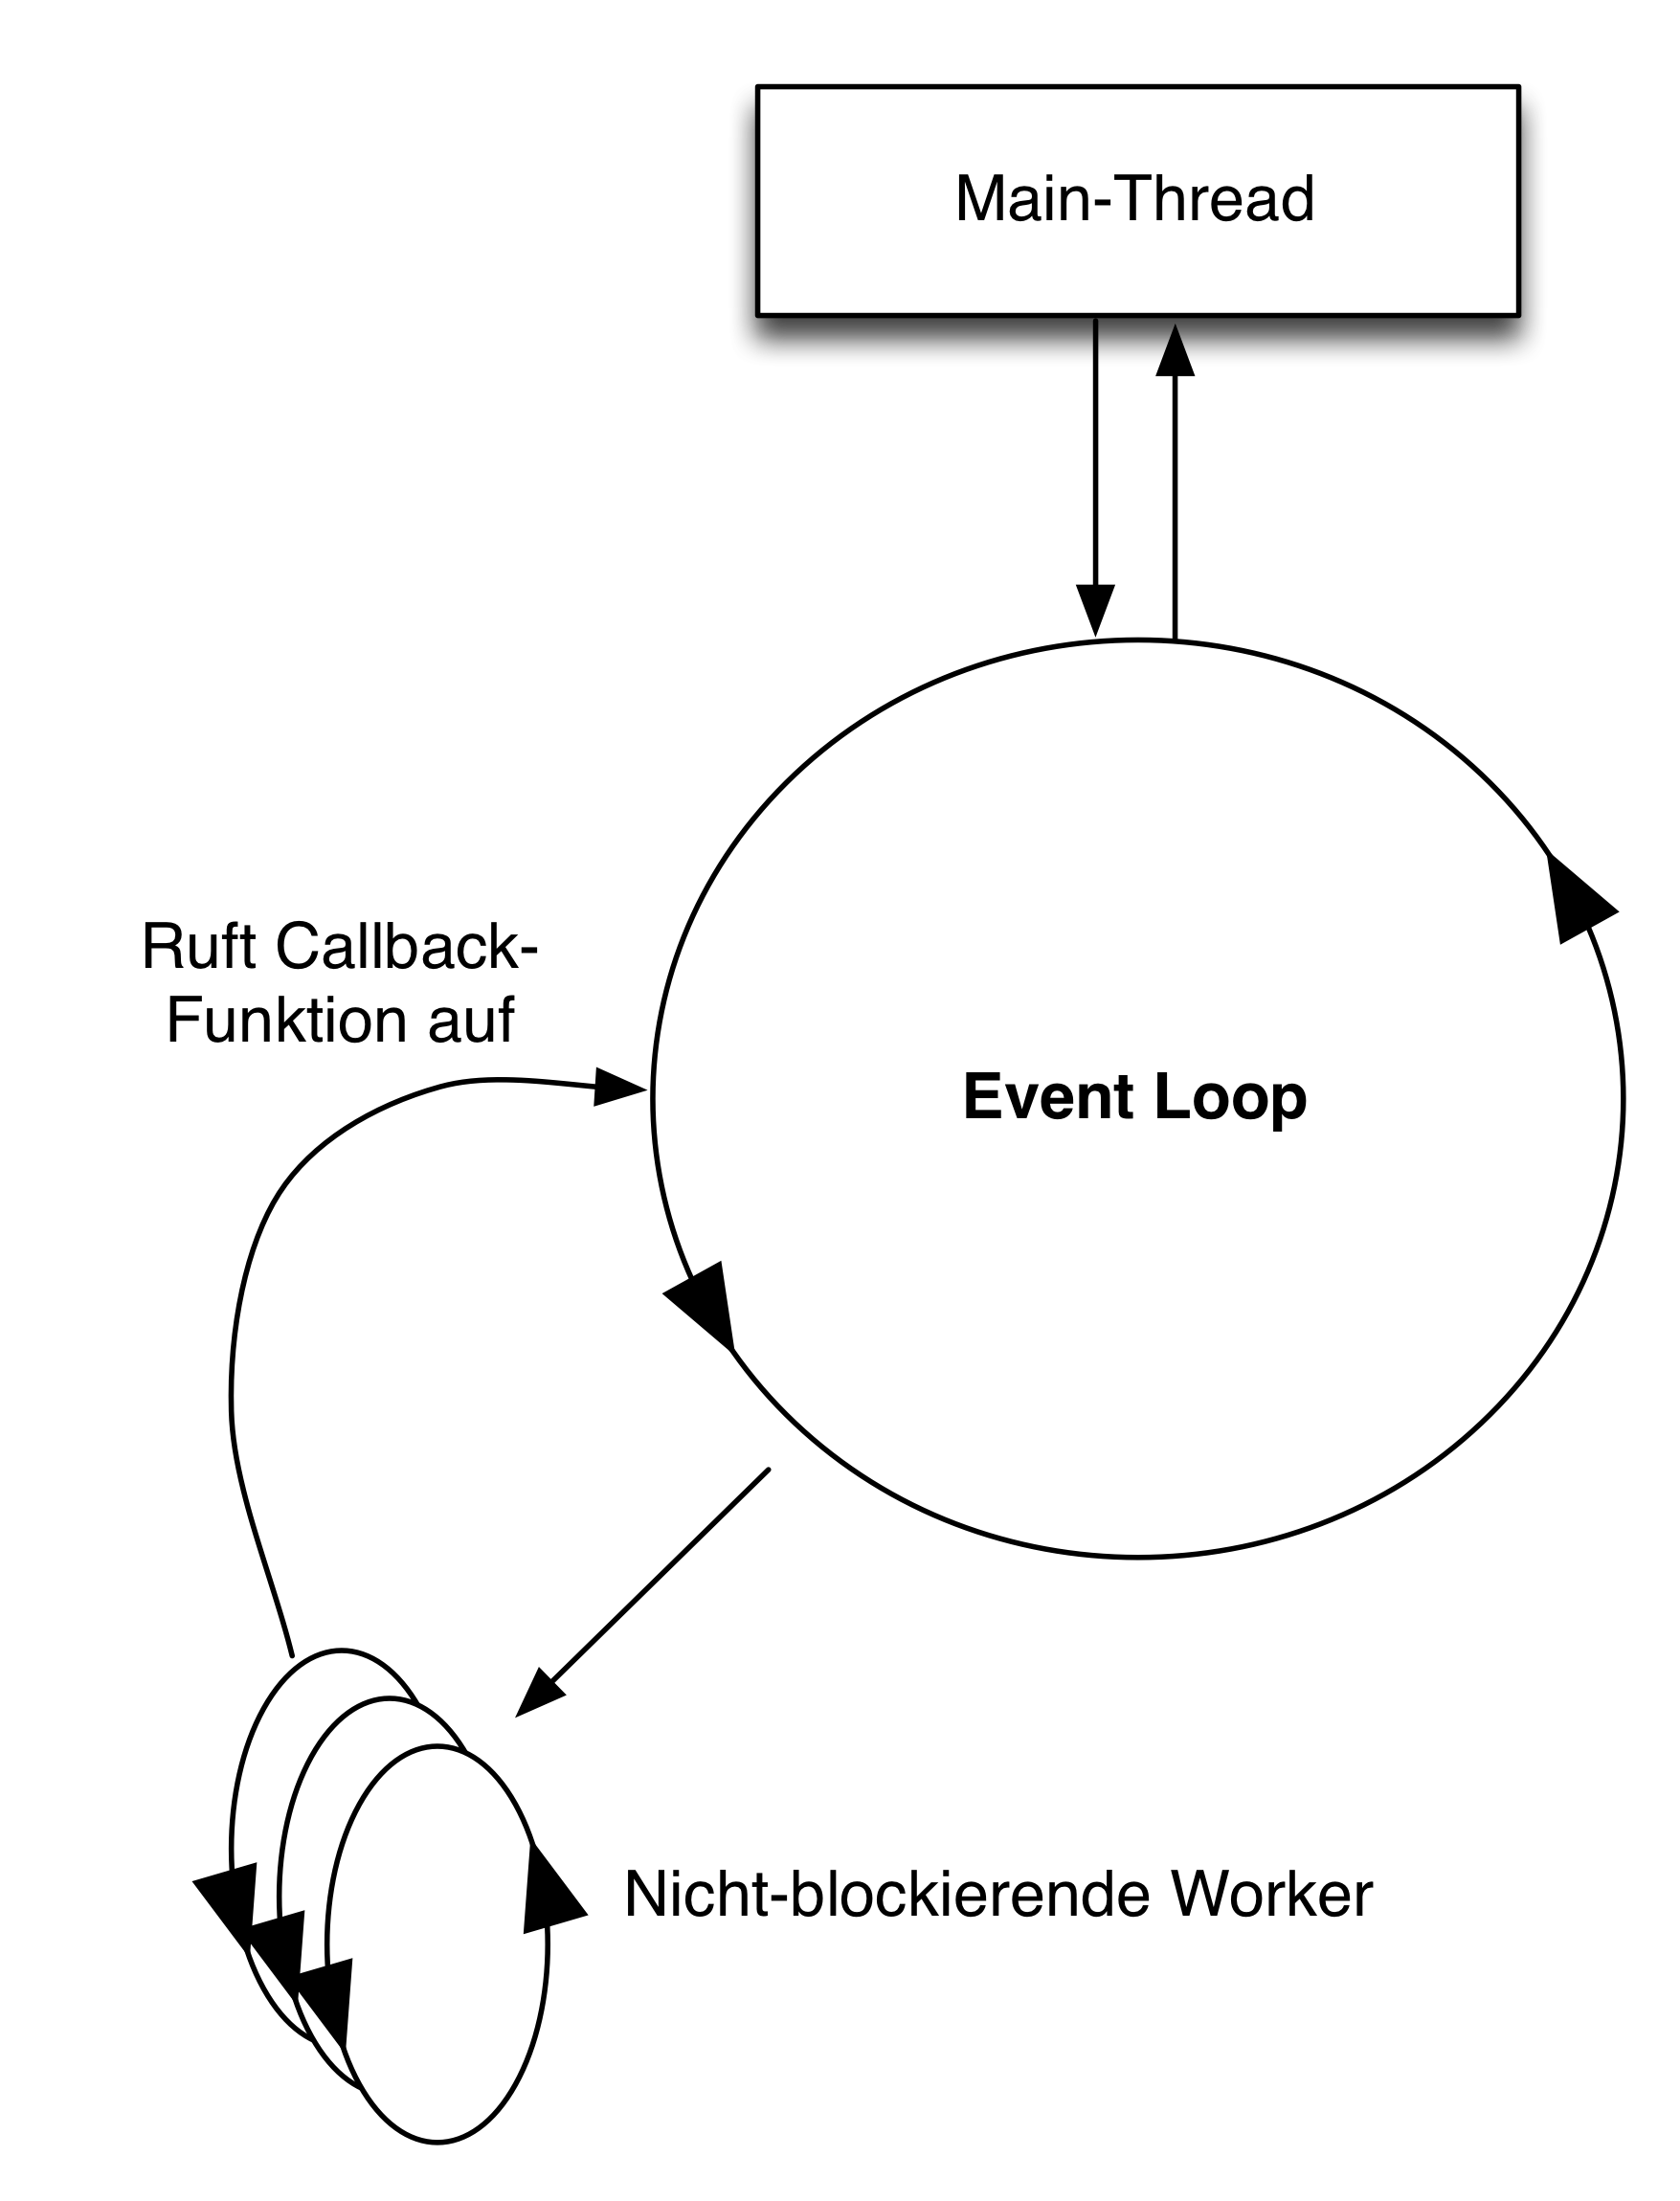
\includegraphics[width=0.4\textwidth]{images/nonblocking.png}
\caption[Event-Loop]{Event-Loop}
\label{fig:nonblocking}
\end{figure}
\acresetall


%Section CSP
\section{\acl{CSP}}
\acf{CSP} ist eine von \textit{C.A.R. Hoare} in seinem Paper\footcite{CSP} \textit{Communication Sequential Processes} 1978 erstmals vorgestellte formale Beschreibung von gleichzeitigen Prozessen und deren Kommunikation untereinander mit Events und Nachrichten.

Als Begründung, warum er ein solches System definiert hat, gibt Hoare an, dass in Zukunft neue Algorithmen benötigt werden, die parallel ausgeführt werden. Durch die zwingende Kommunikation unter den Prozessen ist ein neues Konzept von Nöten, dass das genau spezifiziert und somit die  Effizient steigert. Die damalige Synchronisation über \textit{shared Storage} hat ihm nicht gefallen, da sie zu fehleranfällig und zu komplex war.\footcite[Introduction]{CSP}

Die verwendeten Symbole werden von \textit{C.A.R. Hoare} in seinem Buch\footcite[Glossary of Symbols]{CSPBOOK} beschrieben und können da nachgeschlagen werden.
\subsection[Operatoren und Konstrukte in \acs{CSP}]{Operatoren und Konstrukte in \acs{CSP}\footcite[Siehe][Kap. 1.1]{CSPBOOK}}

Hoare definiert sehr viele Operatoren und Konstrukte. Die Essentiellen von ihren werden nun erläutert. Für Beispiele, wird das von Hoare gerne in seinem Buch\footcite{CSPBOOK} verwendete Beispiel eines Schokoladenautomaten verwendet, jedoch wurden die Begriffe ins Deutsche übersetzt.

\subsubsection{Events}
Events sind Aktionen, die auftreten können. Zwischen eingehenden und ausgehenden Events wird nicht unterschieden. In Hoares Notation werden Events in Kleinbuchstaben geschrieben.
Zum Beispiel bei einem einfachen Schokoladenautomaten gäbe es folgende Events:

\begin{addmargin}[1cm]{0cm}
münze - Das Einwerfen einer Münze in den Automaten.\\
schokolade - Das Entnehmen der Schokolade aus dem Auswurf des Automaten.
\end{addmargin}

Um den Bezug zu \CA\ herzustellen, erweitern wir die Events um Channels, womit sich Hoare erst in einem späteren Kapitel\footcite[Kap. 4.2]{CSPBOOK} im Buch befasst. Stellen wir uns nun den Münzeinwurf (\textit{in}) und den Auswurf (\textit{out}) des Automaten als Channel vor. Die Events aus Sicht des Prozesses sehen nun wie folgt aus:

\begin{addmargin}[1cm]{0cm}
in.münze - Das Entnehmen einer Münze aus dem Münzeinwurf.\\
out.schokolade - Das Hineinlegen einer Schokolade in den Auswurf.
\end{addmargin}

Um Variablen ins Spiel zu bringen gibt es den ?-Operator und den !-Operator. Da das Beispiel dafür ungeeignet ist, wird ein Neues definiert. Nun gibt es einen Automaten (\textit{COPY}), der aus seinem in-Channel liest und den Wert in seinen out-Channel schreibt. Folgende Events gäbe es:

\begin{addmargin}[1cm]{0cm}
in?x - Das Entnehmen von Irgendwas aus dem in-channel und das Speichern in der Variable x.\\
out!x - Das Hineinlegen von dem Wert in der Variable x auf den out-channel.
\end{addmargin}

Alle weiteren Konstrukte werden anhand von Channels erklärt.

\subsubsection{Prozesse}
Ein Prozess definiert sich durch eine Kombination aus verschiedenen Events, die sequentiell hintereinander ausgeführt werden. In unserem ersten Beispiel existiert nur ein Prozess und zwar der Schokoladenautomat \textit{SA}, der durch die Großbuchstaben auch als solches erkenntlich ist. Um einen Automaten terminierbar darzustellen kann nicht einfach nach einem Event nichts mehr folgen, da das die Notation nicht vorsieht. Nach einem Event muss immer ein Prozess oder ein weiteres Event kommen. Deswegen wird hierzu ein Prozess \textit{STOP} definiert, der nach der eigentlichen Ausführung kommt. Er symbolisiert, dass der Schokoladenautomat nicht mehr funktioniert.

\subsubsection{Verkettung}
Um Events, Prozesse und andere Konstrukte sequentiell auszuführen kann $ (\text{in.münze} \rightarrow (out.schokolade \rightarrow STOP)) $ geschrieben werden. Diese Ausführung beschreibt einen Schokoladenautomaten, der eine Münze annimmt und Schokolade auswirft und dann nicht mehr funktioniert. Folgendes hätte auch geschrieben werden können $ SA = (\text{in.münze} \rightarrow \text{out.schokolade} \rightarrow STOP) $. Die Klammern können somit weggelassen werden und der Prozess kann benannt werden.

\subsubsection{Rekursion}
Um nicht den gesamten Ablauf einen Prozesses modellieren zu müssen gibt es Rekursion. Der nicht terminierende Automat \textit{SA} würde wie folgt aussehen:
\begin{addmargin}[1cm]{0cm}
$SA = (\text{in.münze} \rightarrow \text{out.schokolade} \rightarrow SA)$
\end{addmargin}

Das zweite Beispiel eines kopierenden Automaten (\textit{COPY}) sähe wie folgt aus:

\begin{addmargin}[1cm]{0cm}
$COPY = (\text{in?x} \rightarrow \text{out!x} \rightarrow COPY)$
\end{addmargin}

\subsubsection{Parallelität}
\comment{Umschreiben: Ist Kernelement wirklich die parallele Ausführung von mehreren Prozessen?}
Momentan kann die vorgestellte Notation nur einen Prozess ausführen. Jedoch ist das Kernelement von \ac{CSP} die gleichzeitige Ausführung von Prozessen. Bei der gleichzeitigen Ausführung werden Events, die in beiden Alphabeten vorkommen synchron ausgeführt und Events, die nur in einem Prozess vorkommen von dem anderen Prozess ignoriert. Der Operator, der Prozesse parallel ausführt ist der ||-Operator. Definieren wir nun zwei Prozesse.

\begin{addmargin}[1cm]{0cm}
$mensa:SA = \mu X \bullet (\text{in.münze} \rightarrow \text{out.schokolade} \rightarrow X)$\\\\
$student:KUNDE = \mu X \bullet (\text{geldzählen} \rightarrow \text{mensa.in.münze} \rightarrow \text{mensa.out.schokolade} \rightarrow  X)$\\\\
$ (mensa:SA) || (student:KUNDE) $
\end{addmargin}

Der erste Prozess ist der bekannte Schokoladenautomat. Nun ist es aber eine genaue Instanz mit dem Namen \textit{mensa}. $\mu X$ definiert eine Funktion mit dem Bezeichner X, die dann dem Prozess \textit{SA} zugewiesen wird.
Der zweite Prozess ist ein Kunde mit dem Namen \textit{stundent}, der den Schokoladenautomat bedient. Er benutzt die Channels (Münzeinwurf, Ausgabe) des Schokoladenautomaten und zählt am Anfang sein Geld. Um beide Prozesse nun parallel auszuführen, kommt der oben angesprochene ||-Operator ins Spiel, der das ermöglicht.

\comment{Evt die Umwandlung von 2 Parallelen Prozessen in einen Prozess Zeigen. Wäre interessant im Bezug auf die Statemachine}

\subsubsection{Weitere wichtige Konstrukte}
Die oben vorgestellten Konstrukte reichen aus um einen einfachen Automaten zu definieren, der immer den gleichen Ablauf hat. Jedoch werden bei komplexeren Algorithmen Verzweigungen benötigt, um alternative Abläufe zu modellieren. Hierfür definiert die Notation den |-Operator.

\subsection{Umsetzung der Konstrukte in \CA}
In \CA\ ist ein Prozess eine Sequenz von verschiedenen Befehlen, die entweder durch einen Thread ausgeführt werden können oder in einem \textit{go}-Block in einen Zustandsautomat umgewandelt werden.

Die Kommunikation zwischen mehreren Prozessen funktioniert mit Channels, die mit der Funktion \textit{chan} erzeugt werden können. Das Hineinlegen eines Wertes (Event) wird in der Notation nicht vom Herausnehmen unterschieden, außer das Event soll zwischengespeichert werden, dann gibt es die oben erklärten Operatoren (? und !). In \CA\ wird das Hineinlegen eines Werts in einen Channel wird mit den Funktionen \textit{>!!} (bei der Verwendung von Threads) oder \textit{>!} (in einem \textit{go}-Block) gemacht und das Herausnehmen eines Werts aus dem Channel mit den Funktionen \textit{<!!} und \textit{<!} realisiert.

Alle übrigen Konstrukte, wie Rekursion, Verkettung, Verzweigungen etc. werden durch Clojure bzw. \acl{CLJS} abgebildet.

%Section Asynchrone Programmierung JavaScript
%Wieder aktivieren wenn Tobi die Datei hinzugefügt hat.
\section{\acf{CPS} am Beispiel von JavaScript}
\acf{CPS} beschreibt einen Programmierstil, dem die Fortführung (Continuation) eines Programms an ein Unterprogramm übergeben wird. Zumeist werden die Continuations in Form von Funktionszeigern als Parameter an eine Funktion übergeben. In JavaScript werden diese als Callback-Funktionen bezeichnet. Der Einsatz von \acs{CPS} ermöglicht hier die asynchrone Abarbeitung von Funktionen. Betrachten wir folgendes Beispiel:\\
\begin{lstlisting}
function divides(n, m) {
	return (m % n == 0);
}

function getDividers(n, callback) {
	var dividers = Array();
	for(var i = 0; i<n; i++) {
		if(divides(i, n)) {
			dividers.push(i);
		}
	}
	return dividers;	
}
\end{lstlisting}
\comment{ERLÄUTERUNG}
\acresetall


%Section Asynchrone Programmierung Java
\section{Asynchrone Programmierung in Java}
Die einzige Möglichkeit von Haus aus in Java asynchron Befehle auszuführen geht über Threads.

Die Java-Platform bietet hierzu verschiedene Möglichkeiten an, um die Threads einfach zu handhaben. Beispiele dafür sind \textit{Executor}-Framework, \textit{Future}s oder die gerne in der \acs{GUI}-Programmierung verwendeten Callbacks (\textit{Listener}).

\subsection{Threads}

\begin{lstlisting}[language=Java,caption=Definition und Erzeugung eines Threads,label=lst:java_thread]
public class Worker implements Runnable {
	public void run(){
		//Do something asynchronous 	
	}
}
...
gatherInformation();
new Thread(new Worker()).start(); 
continueWork();
\end{lstlisting}


\subsection{ExecutionServices}

\begin{lstlisting}[language=Java,caption=Verwendung eines ExecutionServices,label=lst:java_executionservice]
ExecutorService es = Executors.newFixedThreadPool(2);
gatherInformation();
es.execute(new Worker())
continueWork();
\end{lstlisting}

ForkJoinPool für Rekursive Tasks

\subsection{Callbacks und Futures}
\comment{Callbacks bei UI werden asynchron , bzw später ausgeführt.}
\begin{lstlisting}[language=Java,caption=Verwendung von Futures,label=lst:java_futures]
public class Task implements Callable<Integer> {
	public Integer call(){
		//Do something asynchronous
		return 42; 	
	}
}
...
ExecutorService es = Executors.newFixedThreadPool(2);
gatherInformation();
Future<Integer> f = es.submit(new Task())
continueWork();
...
System.out.println("meaning of life: " + f.get());


\end{lstlisting}
Beide bringen das Ergebnis zurück

\comment{Hier auch Futures erklären}

\subsection{JCSP}

\subsection{Brainstorming}
JCSP, Future, Callback, ExecutionService (bzw nur Executor), Threads







\chapter{Die Bibliothek core.async}

%Section Idee Google GO
\section{Google Go}
Der Ursprung von \textit{go}-Blocks lässt sich auf die von Google entwickelte Programmiersprache \textit{Go} zurückführen. 
\acresetall


%Section API_Beispiele
\section{\acs{API} Code-Beispiele}
Dieses Kapitel demonstriert die Basis-Funktionalität des Frameworks anhand von Code-Beispielen. Zwecks Vereinfachung der Beispiele wird Eingangs die Funktion \textit{read-chan} aus Listing \ref{lst:readchan}\ definiert, die eine einheitliche Ausgabe der Werte auf dem ihr übergebenen Channel realisiert. Diese Funktion durchläuft mit \textit{loop} und \textit{recur} solange alle Werte auf einem Channel, bis dieser geschlossen wird. Das Schließen des Kanals wird durch die Publikation des Wertes \textit{nil} signalisiert.
\begin{lstlisting}[language=Clojure,caption=\textit{read-chan} Hilfsfunktion,label=lst:readchan]
(defn read-chan
  ([c] (read-chan "" c))
  ([str c]
  (thread
    (loop [val (<!! c)]
      (when (not= val nil)
        (println str val)
        (recur (<!! c))))
      (println "END."))))
\end{lstlisting}
\subsection{\textit{Go}-Blocks}
Das folgende Code Beispiel aus Listing \ref{lst:goblock}\ demonstriert den Parking-Mechanismus. Zu Beginn wird  ein ungepufferter Channel \textit{c} erzeugt. Anschließend wird mittels \textit{>!} und \textit{<!} in Kombination mit \textit{go} darauf zugegriffen. Ist der Channel belegt, so wird die \textit{>!} Funktion geparkt. Ein ähnliches Verhalten ist bei \textit{<!} erkennbar, welche geparkt wird, wenn kein Wert auf dem Channel vorliegt. Ist ein Wert vorhanden, so wird dieser vom Channel entfernt und auf der Konsole ausgegeben.
\begin{lstlisting}[language=Clojure,caption=\textit{Go}-Blocks,label=lst:goblock]
(let [c (chan)]
  (go
    (>! c "test"))
  (go
    (println (<! c))))
\end{lstlisting}
\subsection{Threads}
Das obige Beispiel aus Listing \ref{lst:goblock}\ lässt sich auch mit blockierenden Funktionen in Threads ausführen. Die Korrelate zu den Put- und Take-Operation sind hier \textit{>!!} und \textit{<!!}, welche den jeweiligen Thread, in dem sie ausgeführt werden beim Lesen bzw. Schreiben blockieren (siehe Listing \ref{lst:thread}).
\begin{lstlisting}[language=Clojure,caption=Thread,label=lst:thread]
(let [c (chan)]
  (thread
    (>!! c "test"))
  (thread
    (println (<!! c))))
\end{lstlisting}
\subsection{Timeout}
Channels lassen sich in ihrer Lebensdauer zeitlich beschränken, indem man ihre Erzeugung mit Hilfe der \textit{timeout}-Funktion vornimmt. Diese Kanäle werden nach Ablauf des Timeouts automatisch geschlossen. Das folgende Beispiel aus Listing \ref{lst:timeout} demonstriert dieses Verhalten:\\
Zu Beginn wird ein Channel mittels \textit{timeout} erzeugt und neuer Wert asynchron mit Hilfe von \textit{put!} darauf abgelegt. In einem Thread werden nun, wie in der Funktion \textit{read-chan} aus Listing {lst:readchan}\ solange Werte vom Channel abgerufen, bis dieser seine Schließung mittels \textit{nil}-Wert signalisiert.
\begin{lstlisting}[language=Clojure,caption=Timeout,label=lst:timeout]
(let [c (timeout 4000)]
  (put! c "test")
  (thread
  (loop [val (<!! c)]
    (when (not= val nil)
      (println val)
      (recur (<!! c))))
    (println "timeout")))
\end{lstlisting}
\subsection{Filter}
\begin{lstlisting}[language=Clojure,caption=Filter,label=lst:filter]
(let [out (chan)
      c (filter> string? out)]
  (thread
    (>!! c "abc")
    (>!! c 123))
  (read-chan out))
\end{lstlisting}
\subsection{Buffer}
\begin{lstlisting}[language=Clojure,caption=Buffer,label=lst:buffer]
(let [c (chan (buffer 4))]
  (dotimes[n 4]
    (>!! c n))
  (dotimes[n 4]
    (println (<!! c))))
\end{lstlisting}
\acresetall


%Section Hoares Beispiele
\section{Beispiele von Hoare zu \acs{CSP}}
Tony Hoare hat in seinem Paper\footcite{CSP} einige Beispiele erläutert, in denen \ac{CSP} angewendet wird. Einige der einfacheren Beispiele wurde in \textit{core.async} implementiert und sind auf Github\footnote{\url{https://github.com/serofax/CSPHoareExamplesCoreAsync}} zu finden.

Hoare teilt seine Beispiele in vier Bereiche. 

\begin{description}
\item[Coroutines]\hfill \\
Koroutinen sind Prozesse, die Daten von einem oder mehreren entgegennehmen und diese dann in meistens veränderter Form ausgeben.

In \CA\ wurden alle Koroutinen umgesetzt und befinden sich in der Datei \textit{coroutines.clj}.
\item[Subroutines and Data Representation]\hfill \\
Subrotinen sind komplexere Prozesse, die aus Koroutinen zusammengesetzt sind und eine komplexere Aufgabe haben, wie z.B. rekursives Berechnen der Fakultät.

Sechs Beispiele definiert Hoare in seinem Paper. In \CA\ umgesetzt wurden lediglich die rekursive Berechnung der Fakultät und einen Divisionsprozess, der aus einem Dividenten und einem Divisor den Quotienten und den Rest errechnet. Diese beiden Beispiele sind in der Datei \textit{subroutines.clj} zu finden.
\item[Monitores and Scheduling] \hfill \\
In diesen Beispielen werden Prozesse definiert, die die Aufgabe eines Monitors übernehmen um den gleichzeitigen Zugriff auf eine oder mehrere Ressourcen zu koordinieren.

Von den Monitorbeispielen wurden der Integer-Monitor umgesetzt und das Beispiel der Dining Philosopers. Die Monitore in diesem Beispiel sind die Gabeln und der Raum. Die Integer-Monitore ist in der Datei \textit{semaphore.clj} zu finden und das Philosophen-Beispiel in der Datei \textit{philosophers.clj}.
\item[Miscellaneous] \hfill \\
Die Beispiele dieses Kapitel ließen sich in keine der oberen drei Kapitel einteilen. Von diesen wurde keines in \CA\ umgesetzt.
\end{description}








\chapter{Fazit}
\comment{SO FAZIT}


\cleardoublepage

% Schluss
\pagenumbering{Roman}
\setcounter{page}{\value{last_roman}}
\chapter*{Abkürzungsverzeichnis}
\addcontentsline{toc}{chapter}{Abkürzungsverzeichnis}
\markboth{Abkürzungsverzeichnis}{Abkürzungsverzeichnis}
\begin{acronym}
%
%ALPHABETISCH SORTIEREN!!!
%
\acro{API}{Application programming interface}
\acro{CLJS}{ClojureScript}
\acro{CPS}{Continuation-passing style}
\acro{CSP}{Communicating sequential processes}
\acro{IO}{Input/output}
\end{acronym}
\phantomsection
\addcontentsline{toc}{chapter}{Glossar}
\printglossary[title={Glossar}]


\phantomsection
\addcontentsline{toc}{chapter}{Abbildungsverzeichnis}
\markboth{Abbildungsverzeichnis}{Abbildungsverzeichnis}
\listoffigures


\phantomsection
\addcontentsline{toc}{chapter}{Tabellenverzeichnis}
\listoftables

%\phantomsection
%\addcontentsline{toc}{chapter}{Listingverzeichnis}
\renewcommand{\lstlistlistingname}{Listingverzeichnis}
\lstlistoflistings
\phantomsection
\addcontentsline{toc}{chapter}{Literaturverzeichnis}
\begin{thebibliography}{-----------------}

\bibitem[ADCC4]{adcc4}
Adobe Systems Incorporated. \textit{CMIS CONNECTOR FOR ADOBE DRIVE 4: TECHNICAL NOTE}, 2012, URL: \url{http://help.adobe.com/en_US/AdobeDrive/4.0/CMIS_Connector_TechNote.pdf} (besucht am 05.06.2013)

\end{thebibliography}




\chapter*{Anhang}
\addcontentsline{toc}{chapter}{Anhang}
\markboth{Anhang}{Anhang}



\end{document}